\documentclass[a4paper]{article}
\usepackage[spanish]{babel}
\usepackage[utf8]{inputenc}
\usepackage{charter}   % tipografia
\usepackage{graphicx}
%\usepackage{makeidx}
\usepackage{paralist} %itemize inline

%\usepackage{float}
%\usepackage{amsmath, amsthm, amssymb}
%\usepackage{amsfonts}
%\usepackage{sectsty}
%\usepackage{charter}
%\usepackage{wrapfig}
%\usepackage{listings}
%\lstset{language=C}

\usepackage[bookmarks = true, colorlinks=true, linkcolor = black, citecolor = black, menucolor = black, urlcolor = blue]{hyperref} 
\usepackage{color} % para snipets de codigo coloreados
\usepackage{fancybox}  % para el sbox de los snipets de codigo

\definecolor{litegrey}{gray}{0.94}

% \newenvironment{sidebar}{%
% 	\begin{Sbox}\begin{minipage}{.85\textwidth}}%
% 	{\end{minipage}\end{Sbox}%
% 		\begin{center}\setlength{\fboxsep}{6pt}%
% 		\shadowbox{\TheSbox}\end{center}}
% \newenvironment{warning}{%
% 	\begin{Sbox}\begin{minipage}{.85\textwidth}\sffamily\lite\small\RaggedRight}%
% 	{\end{minipage}\end{Sbox}%
% 		\begin{center}\setlength{\fboxsep}{6pt}%
% 		\colorbox{litegrey}{\TheSbox}\end{center}}

\newenvironment{codesnippet}{%
	\begin{Sbox}\begin{minipage}{\textwidth}\sffamily\small}%
	{\end{minipage}\end{Sbox}%
		\begin{center}%
		\vspace{-0.4cm}\colorbox{litegrey}{\TheSbox}\end{center}\vspace{0.3cm}}



\usepackage{fancyhdr}
\pagestyle{fancy}

%\renewcommand{\chaptermark}[1]{\markboth{#1}{}}
\renewcommand{\sectionmark}[1]{\markright{\thesection\ - #1}}

\fancyhf{}

\fancyhead[LO]{Sección \rightmark} % \thesection\ 
\fancyfoot[LO]{\small{Aldasoro Agustina, More \'Angel, Zimenspitz Ezequiel}}
\fancyfoot[RO]{\thepage}
\renewcommand{\headrulewidth}{0.5pt}
\renewcommand{\footrulewidth}{0.5pt}
\setlength{\hoffset}{-0.8in}
\setlength{\textwidth}{16cm}
%\setlength{\hoffset}{-1.1cm}
%\setlength{\textwidth}{16cm}
\setlength{\headsep}{0.5cm}
\setlength{\textheight}{25cm}
\setlength{\voffset}{-0.7in}
\setlength{\headwidth}{\textwidth}
\setlength{\headheight}{13.1pt}

\renewcommand{\baselinestretch}{1.1}  % line spacing


% \setcounter{secnumdepth}{2}
\usepackage{underscore}
\usepackage{caratula}
%\usepackage{url}



% ******************************************************** %
%              TEMPLATE DE INFORME ORGA2 v0.1              %
% ******************************************************** %
% ******************************************************** %
%                                                          %
% ALGUNOS PAQUETES REQUERIDOS (EN UBUNTU):                 %
% ========================================
%                                                          %
% texlive-latex-base                                       %
% texlive-latex-recommended                                %
% texlive-fonts-recommended                                %
% texlive-latex-extra?                                     %
% texlive-lang-spanish (en ubuntu 13.10)                   %
% ******************************************************** %



\begin{document}


\thispagestyle{empty}
\materia{Sistemas Operativos}
\submateria{Primer Cuatrimestre 2015}
\titulo{Trabajo Práctico I}
\subtitulo{Scheduling}
\integrante{Aldasoro Agustina}{86/13}{agusaldasoro@gmail.com}
\integrante{More \'Angel}{XXX/XX}{mail}
\integrante{Zimenspitz Ezequiel}{155/13}{ezeqzim@gmail.com}

\maketitle
\newpage

\thispagestyle{empty}
\vfill
\begin{abstract}
En el presente trabajo se describe la problemática de ...
\end{abstract}

\thispagestyle{empty}
\vspace{3cm}
\tableofcontents
\newpage


%\normalsize
\newpage
\section{Parte I}

\subsection{Ejercicio 1: TaskConsola}
\textit{Programar un tipo de tarea TaskConsola, que simular\'a una tarea interactiva. La tarea debe realizar n llamadas bloqueantes, cada una de una duraci\'on al azar entre bmin y bmax (inclusive). La tarea debe recibir tres par\'ametros: n, bmin y bmax (en ese orden) que ser\'an interpretados como los tres elementos del vector de enteros que recibe la funci\'on.}\\

Al momento de ejecutar la tarea \emph{TaskConsola}, lo que realiza nuestro algoritmo es \emph{uso_IO} \textcolor{red}{(sistema operativo???)} n veces, eligiendo cada vez un n\'umero al azar -mediante la funci\'on rand()- entre bmin y bmax.



\subsection{Ejercicio 2: Ejecuci\'on de tres tareas}
\textit{Escribir un lote de 3 tareas distintas: una intensiva en CPU y las otras dos de tipo interactivo (TaskConsola). Ejecutar y graficar la simulaci\'on usando el algoritmo FCFS para 1, 2 y 3 n\'ucleos.}\\

Las tareas utilizadas en el lote de tareas fueron las siguientes:
	\begin{codesnippet}
	\begin{verbatim}
TaskConsola 4 2 7
TaskCPU 3
@3:
TaskConsola 5 1 10
	\end{verbatim}
	\end{codesnippet}

Para los tres casos se consider\'o un costo de una unidad para cambiar de contexto y para cambiar un proceso de n\'ucleo de procesamiento.\\

Los diagramas de Gantt obtenidos fueron los siguientes:\\

 \begin{figure}[h!]
   \begin{center}
 	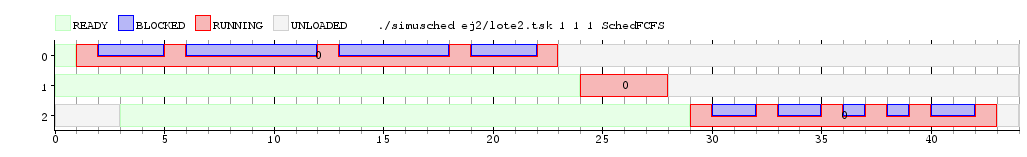
\includegraphics[scale=0.5]{imagenes/ej2/1core.png}
 	\caption{Diagrama de Gantt para la ejecuci\'on del lote de tareas bajo 1 n\'ucleo.}
   \end{center}
 \end{figure} 
 

 \begin{figure}[h!]
   \begin{center}
 	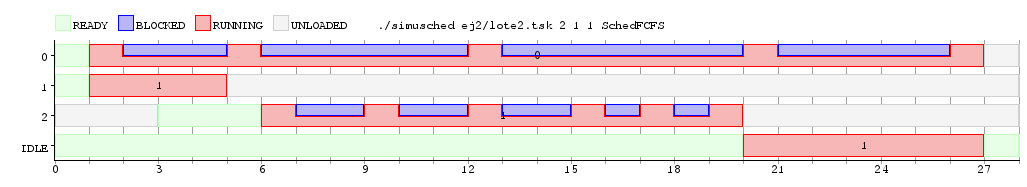
\includegraphics[scale=0.5]{imagenes/ej2/2core.png}
 	\caption{Diagrama de Gantt para la ejecuci\'on del lote de tareas bajo 2 n\'ucleos.}
   \end{center}
 \end{figure} 
 
  \newpage

  \begin{figure}[h!]
   \begin{center}
 	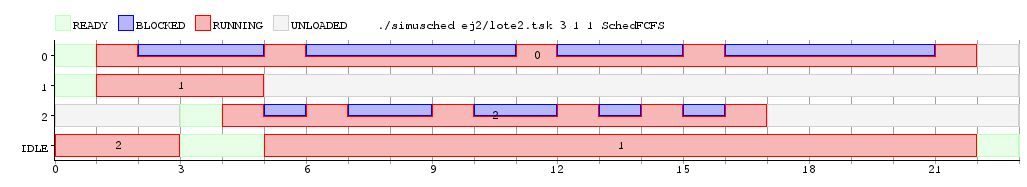
\includegraphics[scale=0.5]{imagenes/ej2/3core.png}
 	\caption{Diagrama de Gantt para la ejecuci\'on del lote de tareas bajo 3 n\'ucleos.}
   \end{center}
 \end{figure} 

\textcolor{red}{Aca habria que hablar un poco :D}

\newpage
\section{Parte II}


\subsection{Ejercicio 3: Scheduler Round-Robin}

\textit{Completar la implementaci\'on del scheduler Round-Robin implementando los m\'etodos de la clase SchedRR en los archivos sched_rr.cpp y sched_rr.h. La implementaci\'on recibe, como primer par\'ametro, la cantidad de n\'ucleos y a continuaci\'on los valores de sus respectivos quantums. Debe utilizar una \'unica cola global, permitiendo as\'i la migraci\'on de procesos entre n\'ucleos.}\\


Las estructuras de datos con las que vamos a trabajar, en la clase \emph{SchedRR}, son las siguientes:
	\begin{codesnippet}
	\begin{verbatim}
		int cores;
		vector<int> quantums;
		vector<int> quantums_timer;
		vector<int> actuales;
		int siguiente;
		queue< int, deque<int> > cola;
	\end{verbatim}
	\end{codesnippet}
	
	\begin{itemize}
	\item[•]\textbf{cores} es la cantidad de n\'ucleos.
	\item[•]\textbf{quantums} es un vector de \textit{cores} posiciones que guarda en quantums[i] el valor del quantum del n\'ucleo i.
	\item[•]\textbf{quantus_timer} es un vector, tal que quantus_timer[i] representa el valor de lo que resta del quantum de la tarea corriendo en el n\'ucleo i. \textcolor{red}{es asi esto que puse?}
	\item[•]\textbf{actuales} son las \textit{cores} tareas que est\'an corriendo ahora. Para la posici\'on actuales[i] ser\'a la tarea que est\'e corriendo en el n\'ucleo i (si no hay nada, sera la Tarea Iddle).
	\item[•]\textbf{siguiente} indica el core que corresponde a utilizar pr\'oximo.
	\item[•]\textbf{cola} es la cola de tareas que restan ser ejecutadas.
	\end{itemize}	
	
%\bigskip	
\noindent  Modificamos a la funcion \emph{next} para que reciba un parametro m\'as (enum Motivo \{ TICK, BLOCK, EXIT \}).
	\begin{codesnippet}
	\begin{verbatim}
    int next(int cpu, const enum Motivo m);
	\end{verbatim}
	\end{codesnippet}
		
\subsubsection*{Constructor Scheduler Round-Robin}		

Al construir un Scheduler Round-Robin, se instancian las estructuras de datos de modo que: se le asigna la cantidad de cores correspondientes (con sus respectivos quantums), todas las tareas actuales se definen como Iddle, la cola est\'a vac\'ia y el siguiente n\'ucleo que le corresponde ejecutar es el primero ingresado como par\'ametro.

\subsubsection*{Funci\'on Load}

Recibo un \emph{pid} como par\'ametro, si tengo alg\'un nucleo libre se la asigno a \'el sino encolo el \emph{pid} en la cola global \emph{cola}. \textcolor{red}{No se porque hace siguiente = cores}

\subsubsection*{Funci\'on Tick}	

\textcolor{red}{El tick pasa para un solo n\'ucleo, cada uno tiene su clock??}.Recibe \emph{cpu} como par\'ametro. S\'olo voy a actualizar el quantum (restarle 1) de la tarea en \emph{cpu} si no es la Iddle, porque esta corre indefinidamente hasta que la desplace otra tarea.

Si se acab\'o el quantum de la tarea actual (ya sea porque termin\'o o no) o se bloque\'o, voy a querer actualizar la tarea actual. Para esto, invoco a la funci\'on \emph{next()}.

Devuelve el \emph{pid} de la tarea actual ejecut\'andose, al pasar el tick del clock.

\subsubsection*{Funci\'on Next}	
	
La funci\'on Next tambi\'en va a ser invocada para un s\'olo n\'ucleo \emph{cpu} pasada por par\'ametro.\\

De este modo, si la tarea que se estaba ejecutando previo a la invocaci\'on de \emph{next()} termin\'o de ejecutarse y la cola se encuentra vac\'ia, la tarea que pondr\'a a ejecutar va a ser la Tarea Iddle.

Si la tarea que se estaba ejecutando no termin\'o su ejecuci\'on o se bloqueo, se deber\'a encolar en la cola global de pendientes.

Si todav\'ia no asign\'e una tarea actual para el n\'ucleo cpu, le asigno la primera de la cola d\'andole todo el quantum disponible para el n\'ucleo \emph{cpu}. (Si la cola se encontraba vac\'ia al llamar la funci\'on next() y la tarea ejecut\'andose no hab\'ia conclu\'ido se la encolar\'a para luego volver a asign\'arsela al n\'ucleo).\\

Devuelve el \emph{pid} de la tarea actual ejecut\'andose.
 
\bigskip 
 
 
 \subsection{Ejercicio 4: Ejecuci\'on de lotes de tareas}
 
\textit{Dise\~nar uno o m\'as lotes de tareas para ejecutar con el algoritmo del ejercicio anterior. Graficar las simulaciones y comentarlas, justificando brevemente por qu\'e el comportamiento observado es efectivamente el esperable de un algoritmo Round-Robin.}\\


Primero ejecutamos el mismo lote de Tareas utilizado anteriormente:
	\begin{codesnippet}
	\begin{verbatim}
TaskConsola 4 2 7
TaskCPU 3
@3:
TaskConsola 5 1 10
	\end{verbatim}
	\end{codesnippet}

	Tambi\'en lo corrimos para 1, 2 y 3 n\'ucleos, cada uno con un quantum de 1, 2 y 3 respectivamente. Para los tres casos se consider\'o un costo de una unidad para cambiar de contexto y para cambiar un proceso de n\'ucleo de procesamiento.\\

Los diagramas de Gantt obtenidos fueron los siguientes:\\


 \begin{figure}[h!]
   \begin{center}
 	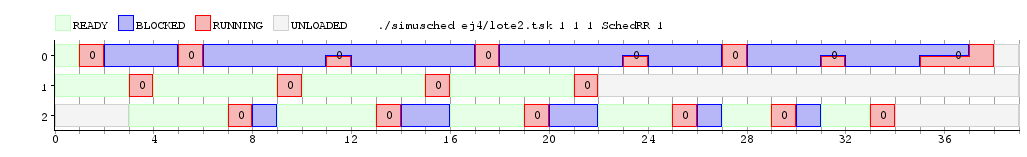
\includegraphics[scale=0.5]{imagenes/ej4/1core.png}
 	\caption{Diagrama de Gantt para la ejecuci\'on del lote de tareas bajo 1 n\'ucleo.}
   \end{center}
 \end{figure} 
 

 \begin{figure}[h!]
   \begin{center}
 	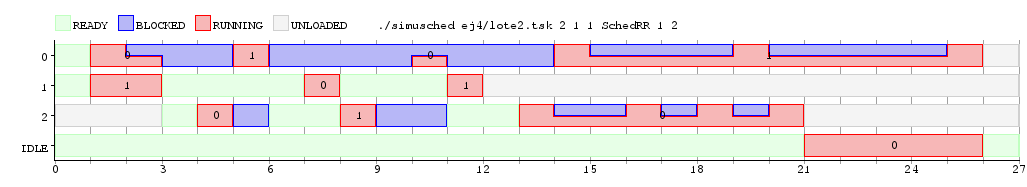
\includegraphics[scale=0.5]{imagenes/ej4/2core.png}
 	\caption{Diagrama de Gantt para la ejecuci\'on del lote de tareas bajo 2 n\'ucleos.}
   \end{center}
 \end{figure} 
 


  \begin{figure}[h!]
   \begin{center}
 	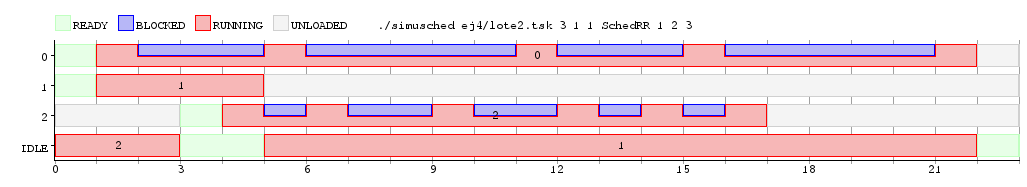
\includegraphics[scale=0.5]{imagenes/ej4/3core.png}
 	\caption{Diagrama de Gantt para la ejecuci\'on del lote de tareas bajo 3 n\'ucleos.}
   \end{center}
 \end{figure} 
 
 \textcolor{red}{Y aca comparamos un poco con como fue la ejecucion antes blablabla}\\
 
 \textcolor{red}{Y aca van otros dos lotes comparando un ejemplo bueno de round robin y uno malo}

\bigskip

 \subsection{Ejercicio 5: Scheduling algorithms for multiprogramming in a hard-real-time environment}
 
\textit{A partir del art\'iculo Liu, Chung Laung, and James W. Layland. Scheduling algorithms for multiprogramming in a hard-real-time environment. Journal of the ACM (JACM) 20.1 (1973): 46-61.}

\begin{enumerate}
\item \textit{Responda:}

\begin{enumerate}
\item \textit{¿Qu\'e problema est\'an intentando resolver los autores?}

The problem of multiprogram scheduling on a single processor is studied from the viewpoint
of the characteristics peculiar to the program function that need guaranteed service. It is shown
that an optimum fixed priority scheduler possesses an upper bound to processor utilization
which may be as low as 70 percent for large task sets. It is also shown that full processor
utilization can be achieved by dynamically assigning priorities on the basis of their current
deadlines. A combination of these two scheduling techniques is also discussed.

\item \textit{¿Por qu\'e introducen el algoritmo de la secci\'on 7? ¿Qu\'e problema buscan resolver con esto?}

We turn now to study a dynamic scheduling algorithm which we call the deadline driven scheduling
algorithm. Using this algorithm, priorities are assigned to tasks according to the deadlines of their
current requests. A task will be assigned the highest priority if the deadline of its current request
is the nearest, and will be assigned the lowest if the deadline of its current request is the furthest.
At any instant, the task with the highest priority and yet fulfilled request will be executed. Such
a method of assigning priorities to the tasks is a dynamic one, in contrast to a static assignment
in which priorities of tasks do not change with time. We want now to establish a necessary and
sufficient condition for the feasibility of the deadline driven scheduling algorithm.

\item  \textit{Explicar coloquialmente el significado del teorema 7.}

For a given set of m tasks, the deadline driven scheduling algorithm is feasible if and
only if\\

(C1/T1) + (C2/T2) + ... + (Cm/Tm) $<=$1:

\end{enumerate}

\item \textit{Dise\~nar e implementar un scheduler basado en prioridades fijas y otro en prioridades din\'amicas. Para eso complete las clases SchedFixed y SchedDynamic que se encuentran en los archivos sched fixed.[h|cpp] y sched dynamic.[h|cpp] respectivamente.}
\end{enumerate}





\newpage
\section{Parte III}


 \subsection{Ejercicio 6: TaskBatch}
\textit{Programar un tipo de tarea TaskBatch que reciba dos par\'ametros: total cpu y cant bloqueos. Una tarea de este tipo deber\'a realizar cant bloqueos llamadas bloqueantes, en momentos elegidos pseudoaleatoriamente. En cada tal ocasi\'on, la tarea deber\'a permanecer bloqueada durante exactamente un (1) ciclo de reloj. El tiempo de CPU total que utilice una tarea TaskBatch deber\'a ser de total cpu ciclos de reloj (incluyendo el tiempo utilizado para lanzar las llamadas bloqueantes; no as\'i el tiempo en que la tarea permanezca bloqueada).}

 \subsection{Ejercicio 7: Ejecuci\'on lote de tareas}
\textit{Elegir al menos dos m\'etricas diferentes, definirlas y explicar la sem\'antica de su definici\'on. Dise\~nar un lote de tareas TaskBatch, todas ellas con igual uso de CPU, pero con diversas cantidades de bloqueos. Simular este lote utilizando el algoritmo SchedRR y una variedad apropiada de valores de quantum. Mantener fijo en un (1) ciclo de reloj el costo de cambio de contexto y dos (2) ciclos el de migraci\'on. Deben variar la cantidad de n\'ucleos de procesamiento. Para cada una de las m\'etricas elegidas, concluir cu\'al es el valor \'optimo de quantum a los efectos de dicha m\'etrica.}

 \subsection{Ejercicio 8: Scheduler Round-Robin modificado}
\textit{Implemente un scheduler Round-Robin que no permita la migraci\'on de procesos entre n\'ucleos (SchedRR2). La asignaci\'on de CPU se debe realizar en el momento en que se produce la carga de un proceso (load). El n\'ucleo correspondiente a un nuevo proceso ser\'a aquel con menor cantidad de procesos activos totales (RUNNING + BLOCKED + READY). Dise\~ne y realice un conjunto de experimentos que permita evaluar comparativamente las dos implementaciones de Round-Robin.}

 \subsection{Ejercicio 9:  Ejecuci\'on lote de tareas}
\textit{Dise\~nar un lote de tareas cuyo scheduling no sea factible para el algoritmo de prioridades fijas pero s\'i para el algoritmo de prioridades din\'amicas.}

 \subsection{Ejercicio 10:  Ejecuci\'on lote de tareas}
\textit{Dise\~nar un lote de tareas, cuyo scheduling s\'i sea factible con el algoritmo de prioridades fijas, donde se observe un mejor uso del CPU por parte del algoritmo de prioridades din\'amicas.}




\end{document}

